\documentclass{article}
	\usepackage[utf8]{inputenc}
	\usepackage{geometry}[top=1cm, right=1cm, left=1cm]
	\usepackage{graphicx}


	\title{Searching: An Exploration of \\ Basic Techniques}
	\author{Trent Baker, Dylan Wickham}

\begin{document}

\maketitle

\section{Introduction}
The problem is to find a path from a starting node in a maze to the goal node. This problem shall be explored on 3 different mazes: one open maze of relatively small size

\section{General Purpose Code}
\subsection{Importing}
The mazes are stored as text files where each character $\in [$`P', `*', `\%', `\ '$]$. Each of these files gets parsed into a 2-D array where each character from the input file becomes a Node (detailed below) that preserves the character and the coordinates. During parsing, if the program reads either `P' or `*', those coordinates are saved for later steps. Once the entire file has been loaded, the program will assign neighbors and calculate distances for each node.

% The run time as O(nm) seems optimal, because how do you import without iterating over the entire maze. However, the space used is inefficient because we could store just the characters in memory initially and then add nodes lazily (as in when we are first about to look at the node, check if it has been made and if not then create the node)


This method is not particularly efficient as implemented, because it contains multiple occurrences or nested for loops making it run in $O(2nm)$ time where $n$ is the width of the input file and $m$ is the height. For this application however, the speed of import is not consequential and even when testing on mazes as large as $2000 \times 2000$ was not causing unacceptable slowdown.

While assigning neighbors, the distance is also calculated to the starting node and to the ending node. These distances are calculated in both Manhattan and euclidean distance, because both metrics are admissible. This simply means that the metric is a lower bound on the total distance a node could be from the relevant location. Not all of the algorithms used these metrics, but because some of them did we decided to pre-calculate the values. This will slow down the import function, but should be a net speed increase because they will not need to be computed on the fly, possibly multiple times.

% I had the above thought about precomputing values in my head when I wrote the function but writing it in the paper now, I realize that if we only calculated the distance when we added it to the open set, we would end up calculating fewer distances overall because unexplored nodes would not need to be calculated. I haven't decided If I want to remove that part or change it yet

\subsection{Node}
The Node class was a simple data structure that allowed us to store all relevant information in one convenient place. Each node has a North, East, South, and West neighbor. If that neighbor is on the border of a maze, the neighbors are simply created as empty nodes with maximal distance. We built checks into all of our algorithms such that they never tried to move into a node with maximal distance from either the start or the goal.

The Nodes were stored in a 2-D array when importing from a file, and must remain in that data structure to be rendered in the end. The search algorithms however, are only given a reference to the starting node. This technique was chosen because it allowed us the possibility of optimization such as tree pruning in the future.

\subsection{Rendering}
Rendering an image is a simple operation and would have been a good addition to this project. We found it beneficial to be able to see the nodes as pixels and colors to differentiate between the different types and states of nodes. This could all be accomplished with text and adding new characters to the maze key as described in the assignment, but for the small amount of effort that generating an image took, the benefits outweighed the consequences. We also experimented with animating the solution by rendering each step in a path as its own frame, but found that apart from the ``cool factor,'' there was not significant benefit. This functionality has been removed from the final code for the sake of clean code, but one of the draft animations has been made available in the repository.

\section{Implemented Algorithms}
\subsection{Depth-First Search (DFS)}
Depth-First Search is a relatively straightforward algorithm to implement. Notables design decisions were using a stack to store nodes on the frontier and finding the path after the search is completed. To avoid a potential stack overflow from recursively calling DFS, a stack of nodes on the frontier was used. Additionally, the path was found after the search was completed. After DFS found the goal, nodes were back traced by going from the goal node and then checking the value of the previous node used in the search to get there. Nodes were then updated to be on the path until the starting node was encountered.
\begin{figure}
	\centering
	\includegraphics[width=0.8\textwidth]{DFS_diagram.png}
	\caption{Depth-First order of discovery}
	\label{fig:dfs_figure}
\end{figure}

% interesting aspects of solution
% non-obvious choices
% parameter settings if applicable
% tips for good performance
% pseudocode? should do for none or all
% figures if neccessary

% MUST INCLUDE:
% renders from all mazes (scaled to width 800px no interpolation)
% path length
% explored nodes

\subsection{Breadth-First Search (BFS)}
Breath-First Search is quite similar to Depth-First Search, with only 2 notables changes needed in the implementation. The first change necessary is quite expected, rather than store the frontier nodes in a stack, a queue was used. The second change was removing duplicate nodes from the frontier, as nodes are not considered visited until they have been pulled from the frontier, this resulted in massive overlaps when exploring the open maze that made it difficult for the algorithm to finish the search.
\begin{figure}
	\centering
	\includegraphics[width=0.8\textwidth]{BFS_diagram.png}
	\caption{Breadth-First order of discovery}
	\label{fig:bfs_figure}
\end{figure}


% interesting aspects of solution
% non-obvious choices
% parameter settings if applicable
% tips for good performance
% pseudocode? should do for none or all
% figures if neccessary

% MUST INCLUDE:
% renders from all mazes(scaled to width 800px no interpolation)
% path length
% explored nodes

\subsection{Greedy Best-First Search (GBF)}

We chose to implement the GBF search with a stack instead of a frontier. This data structure allowed us to easily rebuild the path after arriving at the destination. Each element in the stack was a sorted list of neighbors. While the frontier is also some form of stack, our technique simplifies some of the operations, and was relatively easy to implement. There is some additional overhead, but for the size of the problems we had, this overhead was negligible.

As demonstrated by the open maze path in Figure \ref{fig:greedy_pictures}, this algorithm is not optimal. The paths generated by this algorithm have a tendency to snake back and forth when in certain areas. This is an unfortunate consequence of the algorithm, but is the expected behavior. This snaking occurs when the path must move to nodes with a larger distance to the goal. The algorithm tries to turn all the way around and move directly towards the goal, but because it runs into itself or another visited node, it is forced to turn the other way. This process repeats and creates a snaking path (eventually) to the goal.

The combination of snaking and never reconsidering past decisions means that the paths are generally longer than necessary and not optimal.

% interesting aspects of solution
% non-obvious choices
% parameter settings if applicable
% tips for good performance
% pseudocode? should do for none or all
% figures if necessary
\begin{figure}
	\centering
	\begin{tabular}{c c c}
		& Path Length & Explored Nodes \\
		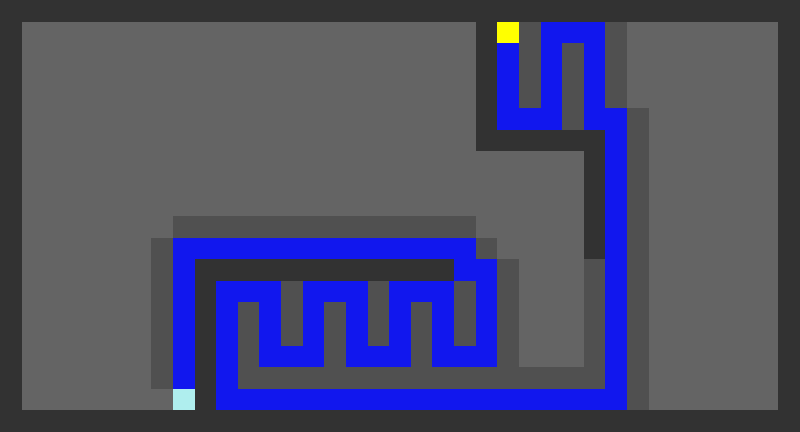
\includegraphics[width=0.4\textwidth]{open_gbf.png} & 107 & 200 \\
		\hline \vspace{-0.1cm} \\
		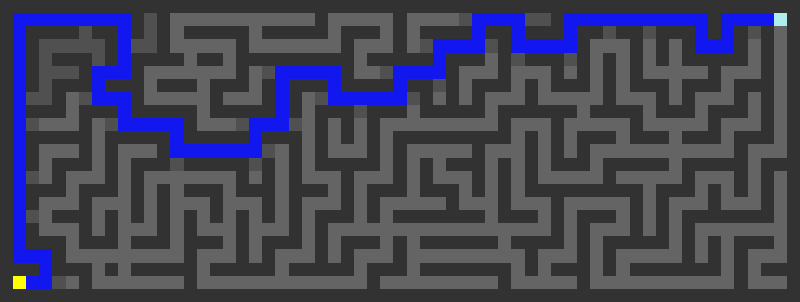
\includegraphics[width=0.4\textwidth]{medium_gbf.png} & 119 & 164 \\
		\hline \vspace{-0.1cm} \\
		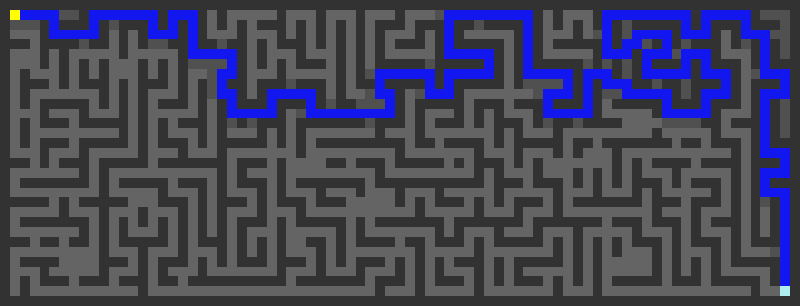
\includegraphics[width=0.4\textwidth]{large_gbf.png} & 235 & 309 \\
		\hline \vspace{-0.1cm} \\
	\end{tabular}

	\caption{Greedy Best-First results}
	\label{fig:greedy_pictures}
\end{figure}


% MUST INCLUDE:
% renders from all mazes(scaled to width 800px no interpolation)
% path length (encoded in filename)
% explored nodes (encoded in filename)

\subsection{A* Search (A*)}
% interesting aspects of solution
% non-obvious choices
% parameter settings if applicable
% tips for good performance
% pseudocode? should do for none or all
% figures if neccessary

% MUST INCLUDE:
% renders from all mazes(scaled to width 800px no interpolation)
% path length (encoded in filename)
% explored nodes (encoded in filename)

\section{Other stuff} %RENAME THIS SECTION
% conclusion as section title?
\subsection{Language Choice}
Kotlin was the chosen language for this experiment, for the language's ability to be concise and that it inter-operates with Java. Kotlin has a variety of design decisions and features that make it much more concise compared to other verbose languages such as Java. The conciseness makes it both faster to develop solutions in but also makes code more readable by greatly limiting the presence of boilerplate code. Additionally, Kotlin inter-operates with Java which allows the use of a relatively new language while having the many supporting libraries of Java for use as needed.
\subsection{Experimental Design}

Because these four algorithms are not particularly complex, a large part of our testing was accomplished simply by looking at the rendered output. We generated many additional mazes, both to test our algorithms in more cases, and to ensure that our algorithms were behaving properly.

\subsection{Algorithm Comparison}
Include images here where all of the algorithms are run on each of the mazes

\begin{figure}
	\centering
	\caption{Caption}
	\label{fig:algorithm_comp}
\end{figure}

\section{Future development}
Tree pruning could be used to simplify the mazes and increase performance. Any given node can have $0-4$ walls as neighbors. If a node has 2, 3, or 4 walls as neighbors, there are no choices to be made. Assuming that at least one non-wall neighbor is  required as the entrance to a node, the above cases are hallways, dead ends, and error states respectively. The remaining cases are the interesting cases where decisions are made, but are the minority in most mazes we looked at. If we were to scan through a maze and prune the graph of nodes that did not present a decision, problem could be drastically simplified. Some mazes however, such as the provided open maze, would only be able to prune a few nodes leading to negligible performance increases.

\end{document}
